\chapter{车道汇合群决策模型仿真}
\label{cha:sim}
% 仿真的一些综述

\section{仿真平台设计}
本课题中使用{\ttfamily Python}开发仿真程序。仿真程序大体框架如图\ref{fig:ss}。
\begin{figure}
\centering
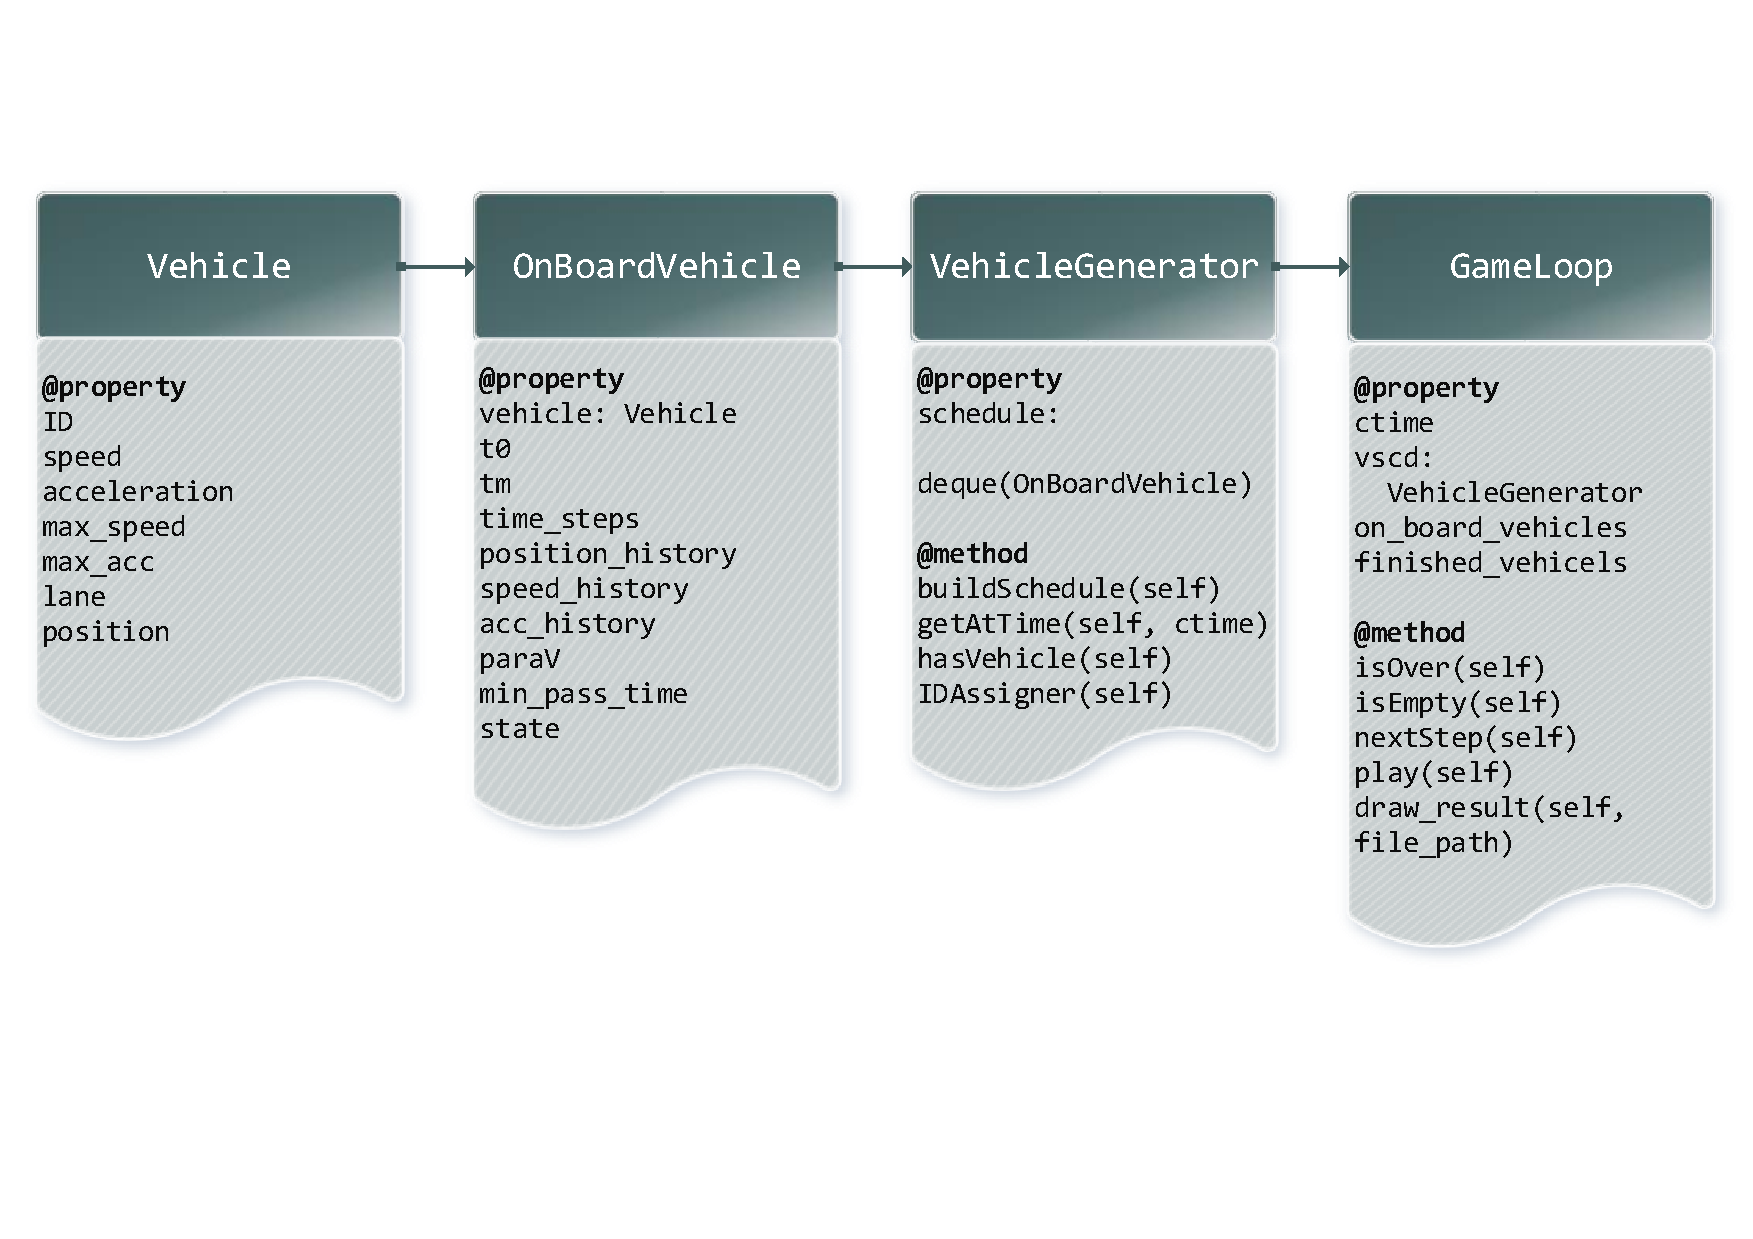
\includegraphics[width=15cm,trim={0 4cm 0 2cm},clip]{figures/software_structure.pdf}
\caption{仿真程序结构}
\label{fig:ss}
\end{figure}

为了方便进行仿真实验展示,本课题使用{\ttfamily Python}的{\ttfamily bokeh}包开发了如图\ref{fig:app}所示的仿真应用程序。
\begin{figure}
\centering
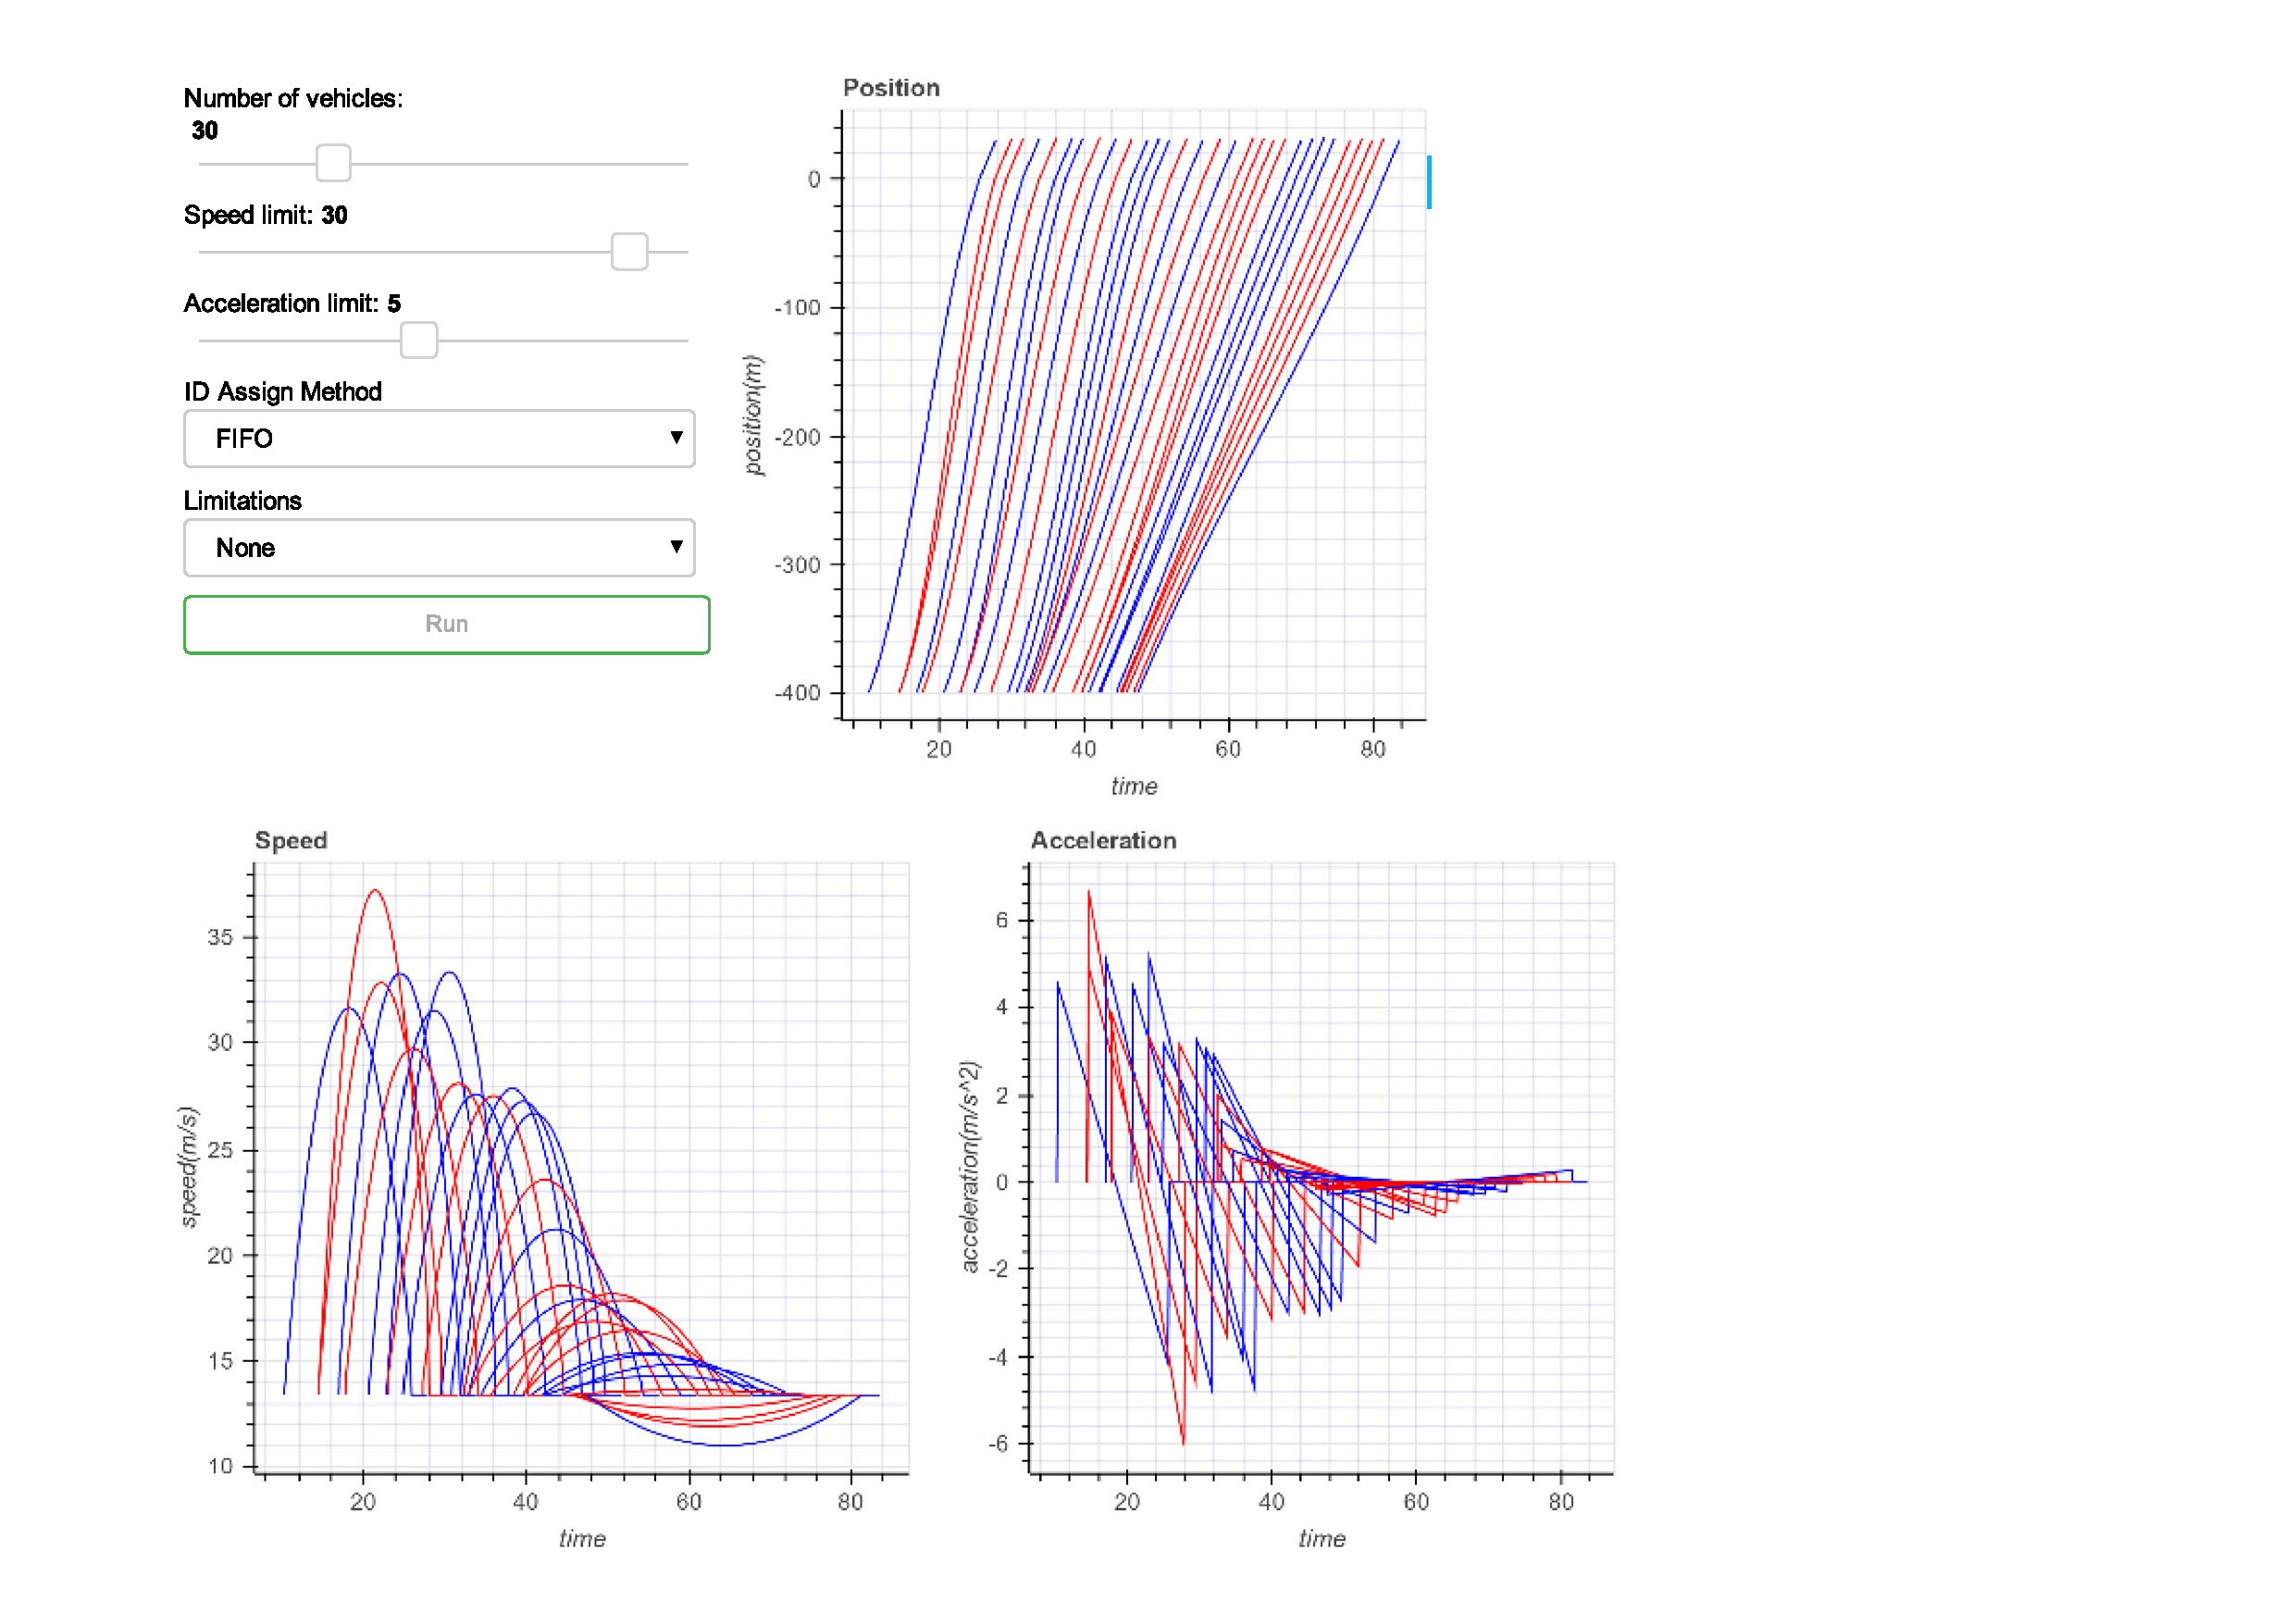
\includegraphics[angle=270,trim={0 0 0 10cm},clip,width=15cm]{figures/app.pdf}
\caption{网页APP仿真平台界面}
\label{fig:app}
\end{figure}

\section{评价指标计算}
\paragraph{}

\section{简单FIFO序列仿真}
\subsection{相同速度进入控制区}
首先检验算法是否能保证车辆进入交汇区不碰撞。不考虑速度和加速度限制,所有车辆以相同速度进入控制区,且从两车道成对进入(同一时刻两车道各有一辆车进入),一共有四辆车。在该情况下,如果不进行控制而匀速运行,两车道的车辆会发生碰撞。仿真参数设置如表\ref{tab:case1:param}。这组实验到达交汇口时间$t_i^\mathrm{m}$由式\ref{eq:tmcase}给出,第一辆车通过时间由式\ref{eq:tmopt}解出。
\begin{table}[htbp]
\centering
\caption{第一组仿真实验参数}
\label{tab:case1:param}
\begin{tabular}{lll}
\toprule[1.5pt]
参数符号 & 参数含义 & 参数值 \\
\midrule[1pt]
$L$ & 控制区长度 & $\SI{400.0}{m}$ \\
$S$ & 交汇区长度 & $\SI{30.0}{m}$ \\
$\delta$ & 安全距离 & $\SI{10}{m}$ \\
$v_0$ & 初速度 & $\SI{13.4}{m\per s}$ \\
$v_\mathrm{d}$ & 期望速度 & $\SI{25.0}{m\per s}$ \\
$t_1^0, t_2^0$ & 一、二号车进入路口时刻 & $\SI{10.0}{s}$ \\
$t_3^0, t_4^0$ & 三、四号车进入路口时刻 & $\SI{15.0}{s}$ \\
\bottomrule[1.5pt]
\end{tabular}
\end{table}

仿真结果如图\ref{fig:case1:posi}---\ref{fig:case1:fuel}。由图可见,
\begin{figure}
\begin{minipage}{0.48\textwidth}
  \centering
  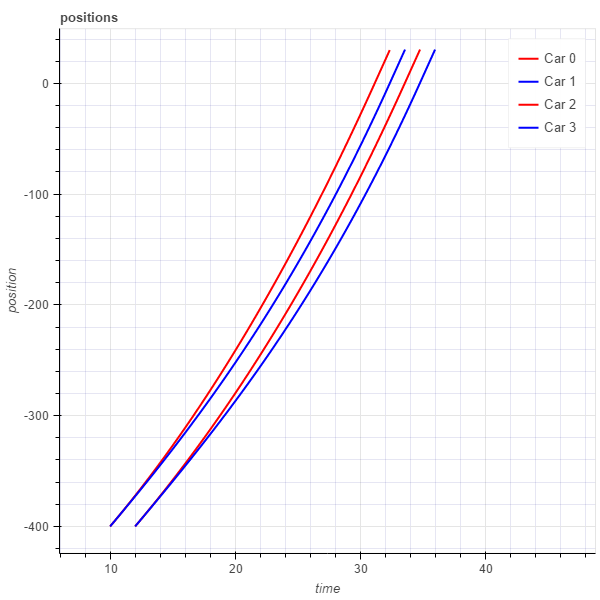
\includegraphics[height=6cm]{figures/sim_case1/posi.png}
  \caption{位移-时间关系图(第一组)}
  \label{fig:case1:posi}
\end{minipage}\hfill
\begin{minipage}{0.48\textwidth}
  \centering
  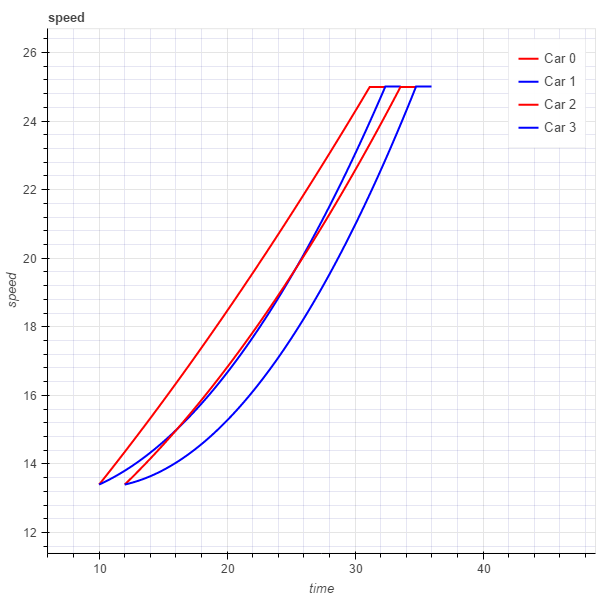
\includegraphics[height=6cm]{figures/sim_case1/speed.png}
  \caption{速度-时间关系图(第一组)}
  \label{fig:case1:speed}
\end{minipage}
\end{figure}
\begin{figure}
\begin{minipage}{0.48\textwidth}
  \centering
  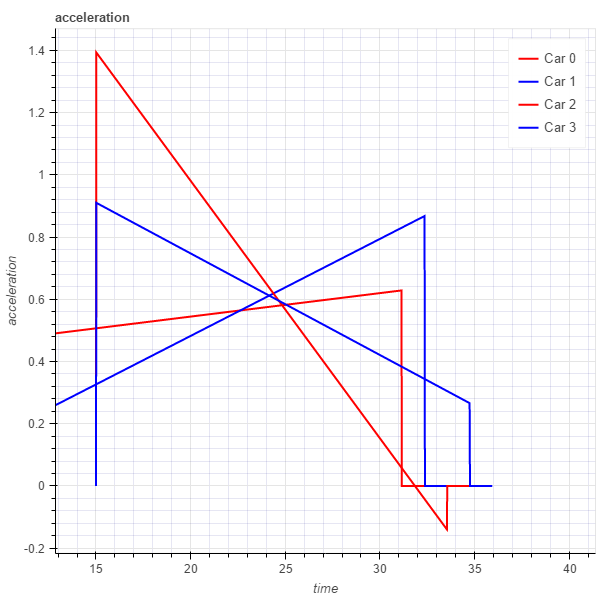
\includegraphics[height=6cm]{figures/sim_case1/acc.png}
  \caption{加速度-时间关系图(第一组)}
  \label{fig:case1:acc}
\end{minipage}\hfill
\begin{minipage}{0.48\textwidth}
  \centering
  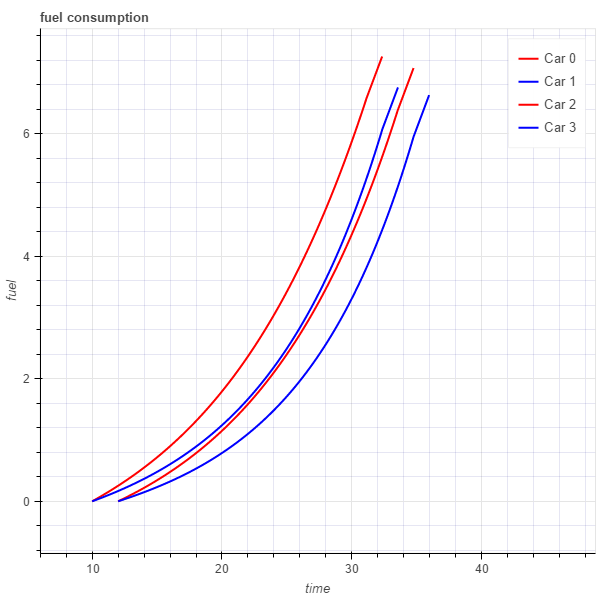
\includegraphics[height=6cm]{figures/sim_case1/fuel.png}
  \caption{油耗-时间关系图(第一组)}
  \label{fig:case1:fuel}
\end{minipage}
\end{figure}

\subsection{主辅路不同速度进入控制区}
\subsection{随机速度进入控制区}

\section{最优通行时间顺序仿真实验}

% \section{改进的优先到达序列仿真}
% \subsection{排序原理}
% \subsection{时间目标优先}
% \subsection{系统能量目标优先}

% \chapter{群决策模型改进}
% (有时候由于信息不准或延迟,可能控制区会撞)
% \section{碰撞紧急修正处理}
% \subsection{修正必要性与原理}
% \subsection{带有修正的系统仿真}
% \section{}